\documentclass{standalone}
\usepackage{tikz}
\usepackage{fontspec}
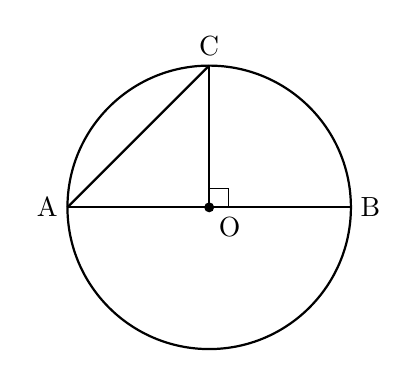
\begin{tikzpicture}[scale=1.2]
    % বৃত্ত ও কেন্দ্র O
    \draw[thick] (0,0) circle (1.5cm);
    \coordinate (O) at (0,0);
    \node[below right] at (O) {O};
    \fill (O) circle (1.5pt);
    
    % ব্যাস AB এবং ব্যাসার্ধ OC অঙ্কন
    \coordinate (A) at (-1.5, 0);
    \coordinate (B) at (1.5, 0);
    \coordinate (C) at (0, 1.5);
    \draw[thick] (A) -- (B);
    \draw[thick] (O) -- (C);
    \draw[thick] (A) -- (C);
    
    % লেবেলসমূহ
    \node[left] at (A) {A};
    \node[right] at (B) {B};
    \node[above] at (C) {C};
    
    % সমকোণ চিহ্ন
    \draw (0, 0.2) -- (0.2, 0.2) -- (0.2, 0);
\end{tikzpicture}
\end{document}
